\documentclass{beamer}
\usepackage{amsmath}
\usepackage{icomma}
\usepackage[utf8]{inputenc}
\usepackage[T1]{fontenc}
\usepackage{polski}
\usepackage[polish]{babel}
\usepackage{hyperref}
\usepackage{float}
\usepackage{textcomp}
\usetheme{Darmstadt}
\usecolortheme{rose}

% Naprawa nazw z angielskiego
\def\figureautorefname{Rysunek}

%Strona streszczenia
\newenvironment{abstractpage}
  {\cleardoublepage\vspace*{\fill}\thispagestyle{empty}}
  {\vfill\cleardoublepage}
  
%Samo streszczenie
\newenvironment{abstractsection}[1]
  {\bigskip\selectlanguage{#1}%
   \begin{center}\bfseries\abstractname\end{center}}
  {\par\bigskip}

%Ładne ułamki w jednostkach fizycznych
\sisetup{per-mode=symbol}%

\beamertemplatenavigationsymbolsempty
\setbeamertemplate{footline}[frame number]

\begin{document}
	\section{Wprowadzenie}
	\begin{frame}
		\title[Omnivelma]{Symulacja dookólnej bazy mobilnej}
		\author{Radosław Świątkiewicz}
		\date{\today}
		\institute{Promotor: dr hab. inż. Wojciech Szynkiewicz \\ \footnotesize Instytut Automatyki i Informatyki Stosowanej \\ Wydział Elektroniki i Technik Informacyjnych \\ Politechnika Warszawska}
		\titlepage
	\end{frame}
	\begin{frame}
		\frametitle{Spis treści}
		\tableofcontents[currentsection]
	\end{frame}
	
	
	
	\section{Problem}
	\begin{frame}
		\frametitle{Roboty}
		\begin{columns}[c]
			\column{0.5\textwidth}
			\centering
			\includegraphics[width=0.8\textwidth]{graphics/velma.png} \\
			Robot manipulacyjny Velma
			\column{0.5\textwidth}
			\centering
			\includegraphics[width=\textwidth]{graphics/omnivelma.png} \\
			Platforma na kołach Mecanum
		\end{columns}
	\end{frame}
	
	\begin{frame}
		\frametitle{Cel projektu --- opracowanie modelu i środowiska symulacyjnego platformy}
		Do czego przydatny jest model:
		\begin{itemize}
			\item Pozwala na bezpieczne testowanie nowego oprogramowania.
			\item Przyspiesza implementację i testowanie programu sterującego.
			\item Pozwala na przeprowadzanie skomplikowanych i niebezpiecznych dla robota testów.
			\item Daje możliwość modelowania czujników niezamontowanych w urządzeniu.
		\end{itemize}
		Wymagania:
		\begin{itemize}
			\item Model reaguje na momenty siły i siły tarcia w sposób zbliżony do robota.
			\item Przyjmuje taką samą postać sygnałów sterujących.
			\item Generuje dane z czujników wirtualnych, zbliżone do rzeczywistych.
		\end{itemize}
	\end{frame}
	
	\begin{frame}
		\frametitle{Założenia}
		\begin{itemize}
			\item Ze względu na ograniczoną moc obliczeniową komputera, modele kół muszą być przybliżone.
			\item Robot i model poruszają się tylko po płaszczyźnie.
			\item Odwzorować należy kinematykę, dynamikę i tarcie.
			\item Mogą występować poślizgi kół.
			\item Symulacja obarczona jest naturalnym numerycznym błędem liczb zmiennoprzecinkowych.
		\end{itemize}
	\end{frame}

	

	\section{Platforma}
	\begin{frame}
		\frametitle{Koła Szwedzkie (Mecanum)}
		\centering
		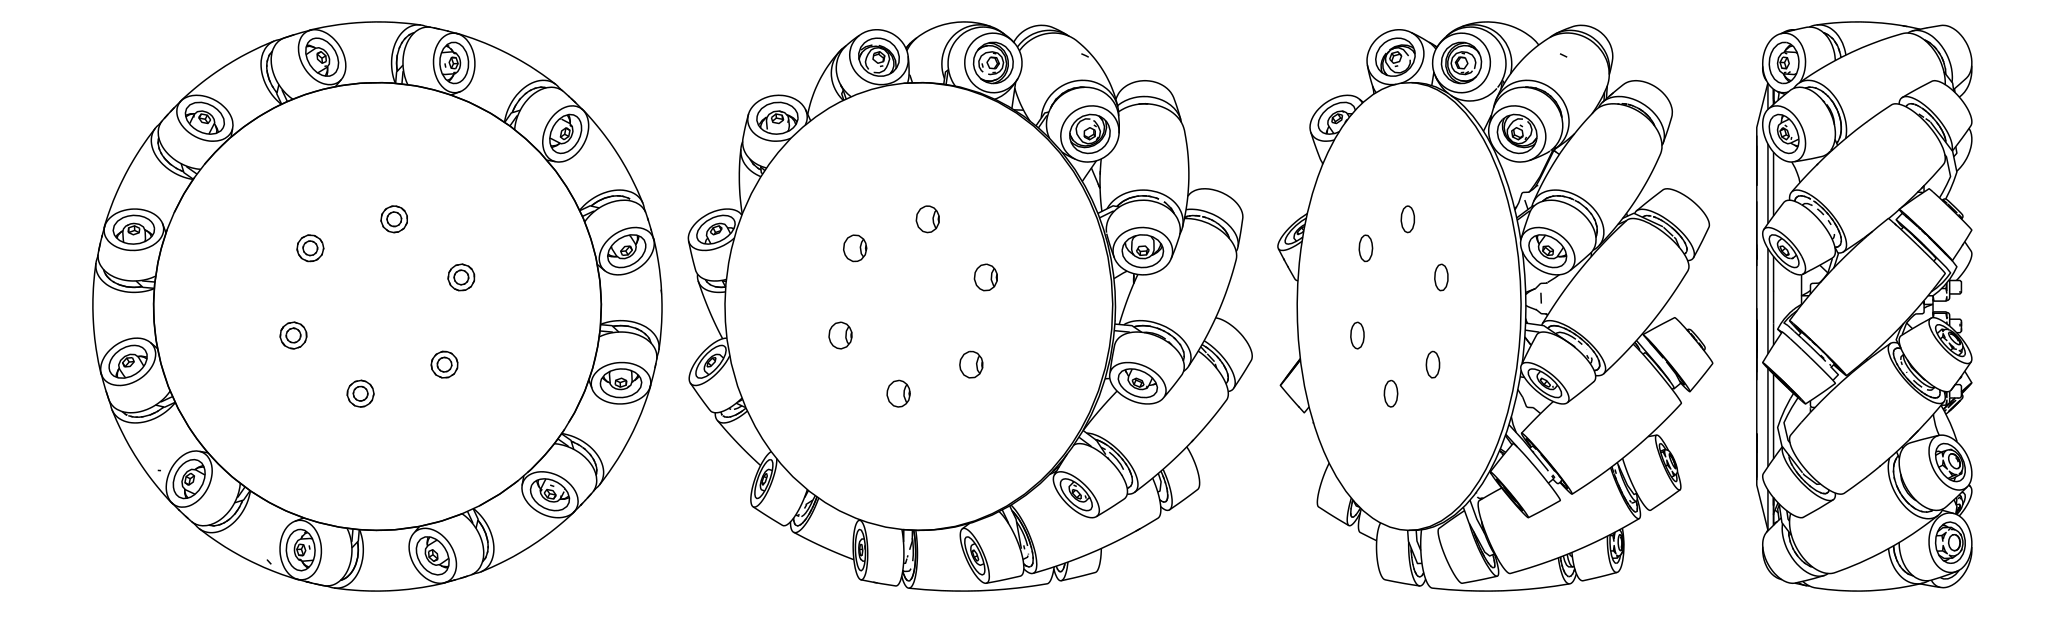
\includegraphics[width=\textwidth]{graphics/wheel.pdf}
		\begin{itemize}
			\item Każde koło ma 12 pasywnych rolek.
			\item Rolka jest obrócona o 45° względem osi obrotu koła.
			\item Punkt kontaktu rolki z podłożem powinien płynnie przechodzić z rolki na rolkę.
			\item Oś rolki aktualnie znajdującej się u góry koła jest prostopadła do osi rolki kolidującej z podłożem.
		\end{itemize}
	\end{frame}
	
	\begin{frame}
		\frametitle{Budowa}
		\centering
		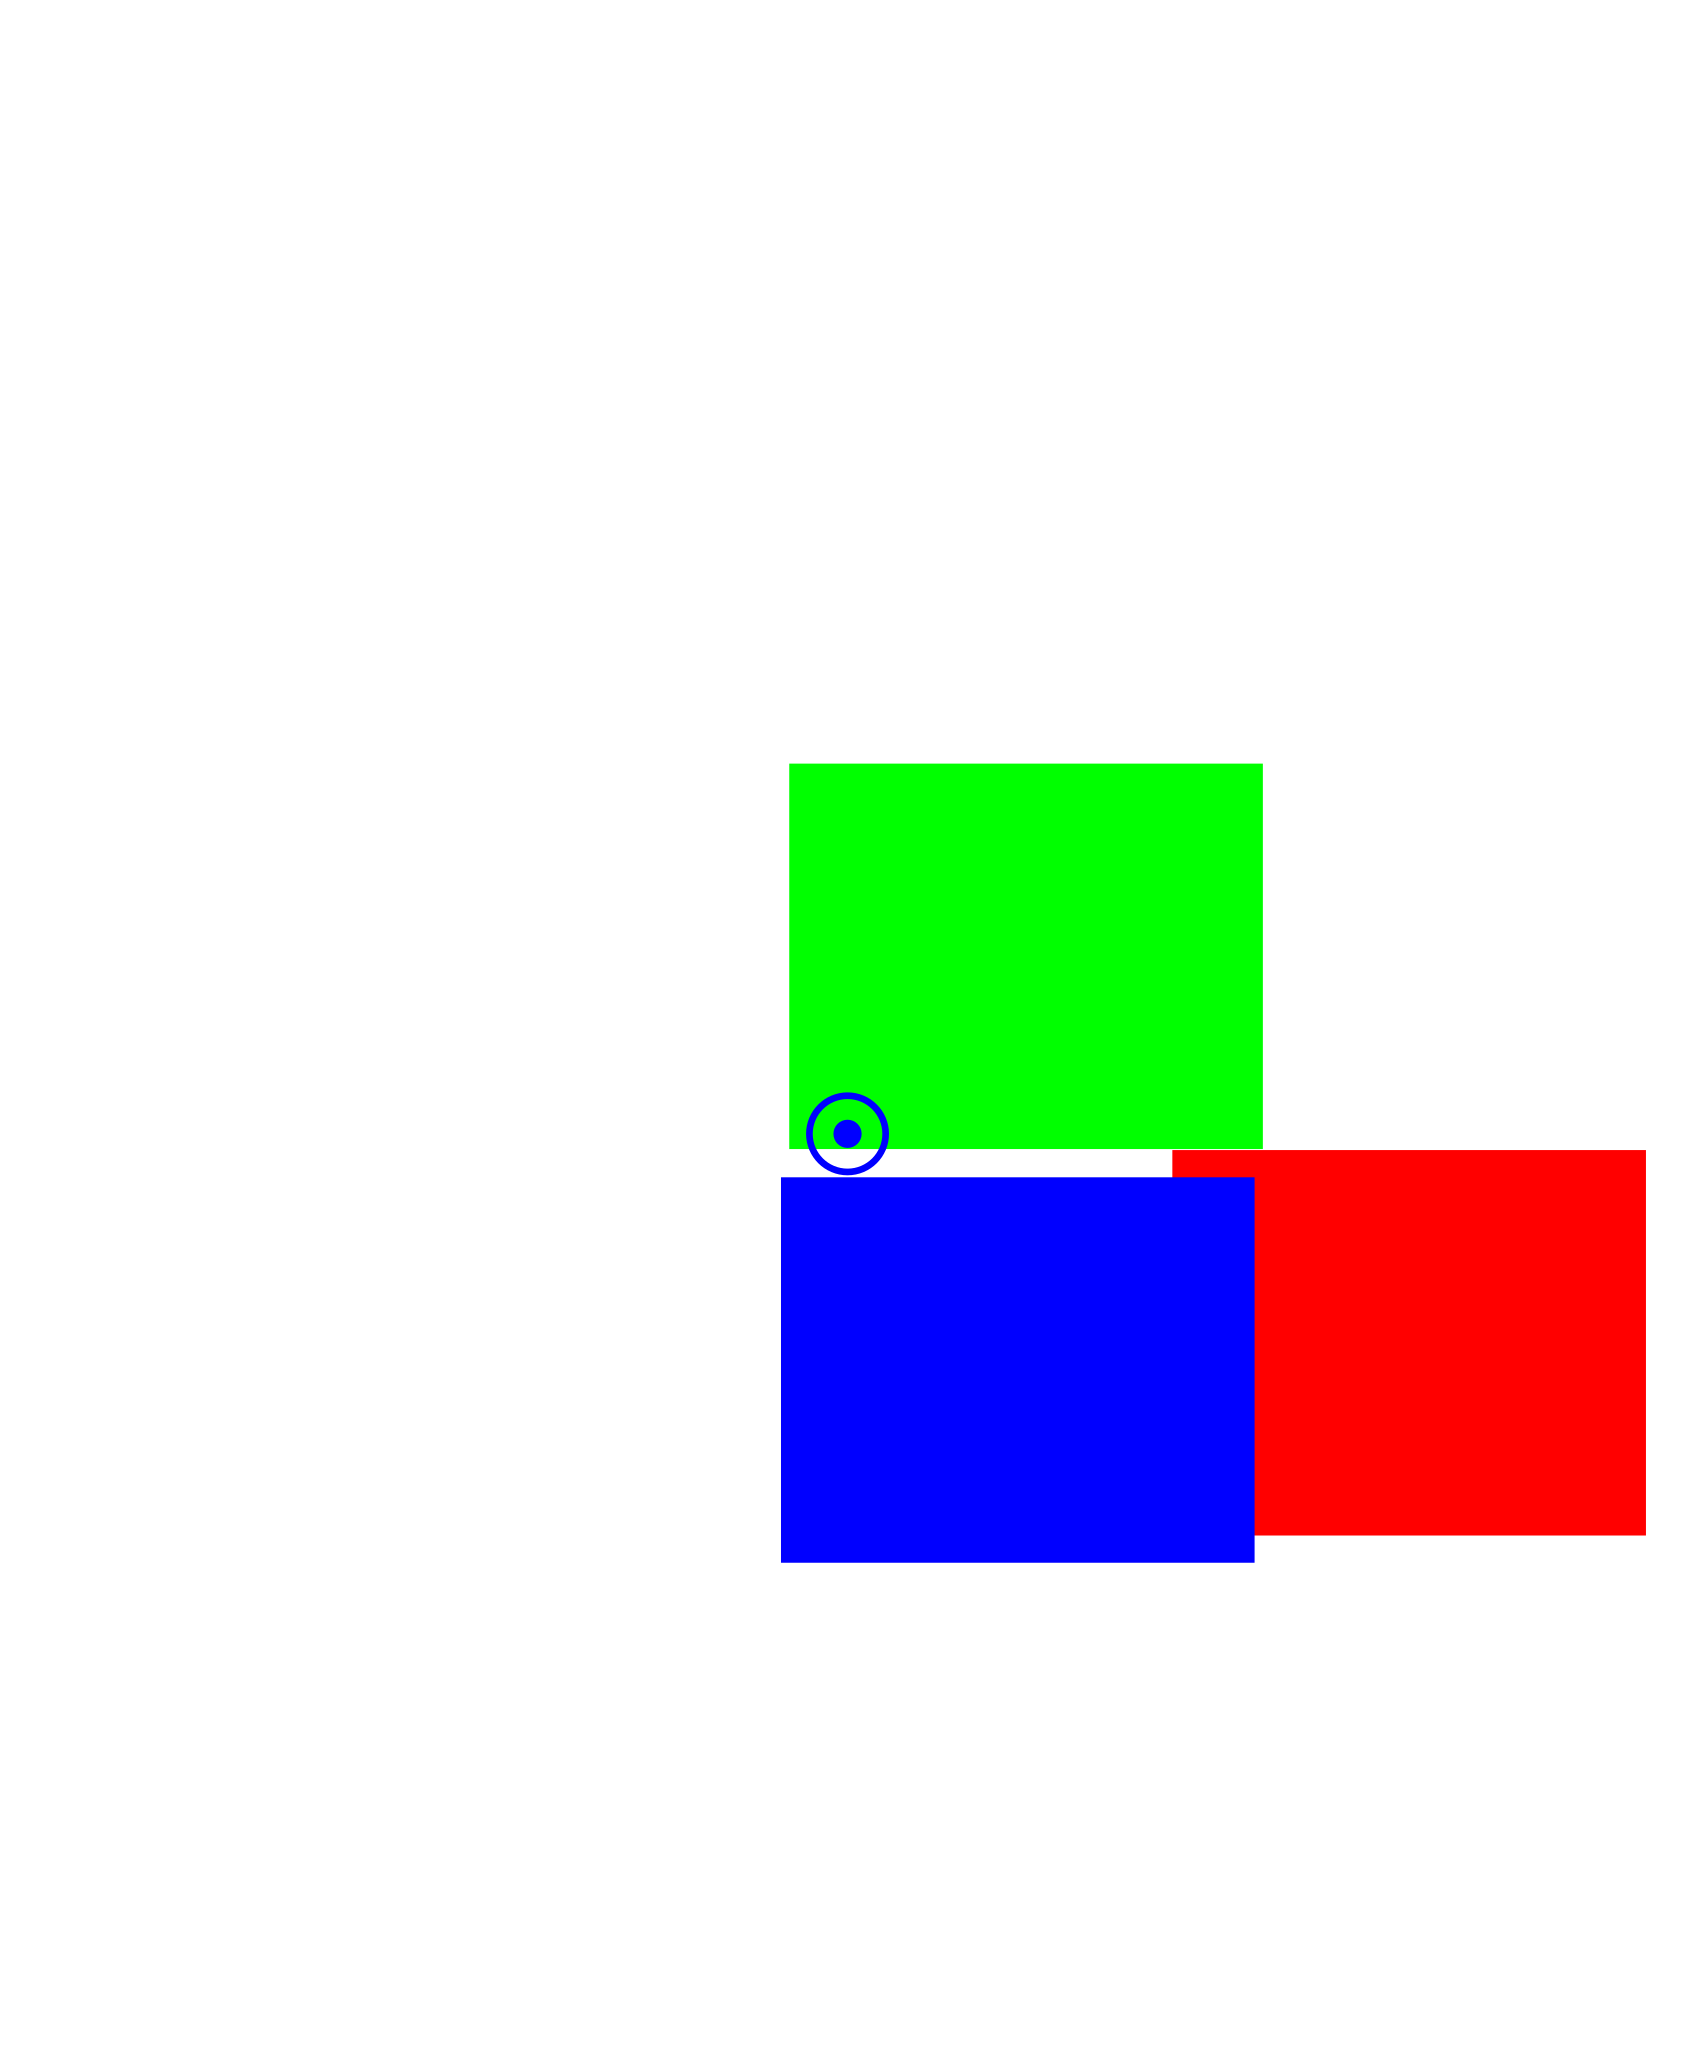
\includegraphics[width=0.4\textwidth]{graphics/base.pdf}
		\begin{itemize}
			\item Koła ustawione są w kształt litery \emph{X}.
			\item Przegub o jednym stopniu swobody łączy dwie części platformy.
		\end{itemize}
	\end{frame}
	
	\begin{frame}
		\frametitle{Kierunki ruchu}
		\centering
		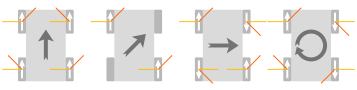
\includegraphics[width=\textwidth]{graphics/mecanum_dirs_vect.pdf} \\
		Poprzez znoszenie się składowych wektorów sił, robot może poruszać się w kierunkach nieosiągalnych dla pojazdów o zwykłych kołach.
	\end{frame}
	
	\begin{frame}
		\frametitle{Model kinematyki}
		\[
		\begin{bmatrix}
		v_x \\
		v_y \\
		\omega_z \\
		\end{bmatrix}
		=
		\frac{r}{4}
		\begin{bmatrix}
		-1 & 1 & -1 & 1 \\
		1 & 1 & 1 & 1 \\
		\frac{2}{a+b} & \frac{-2}{a+b} & \frac{-2}{a+b} & \frac{2}{a+b} \\
		\end{bmatrix}
		\begin{bmatrix}
		\omega_1 \\
		\omega_2 \\
		\omega_3 \\
		\omega_4 \\
		\end{bmatrix}
		\]
		\centering
		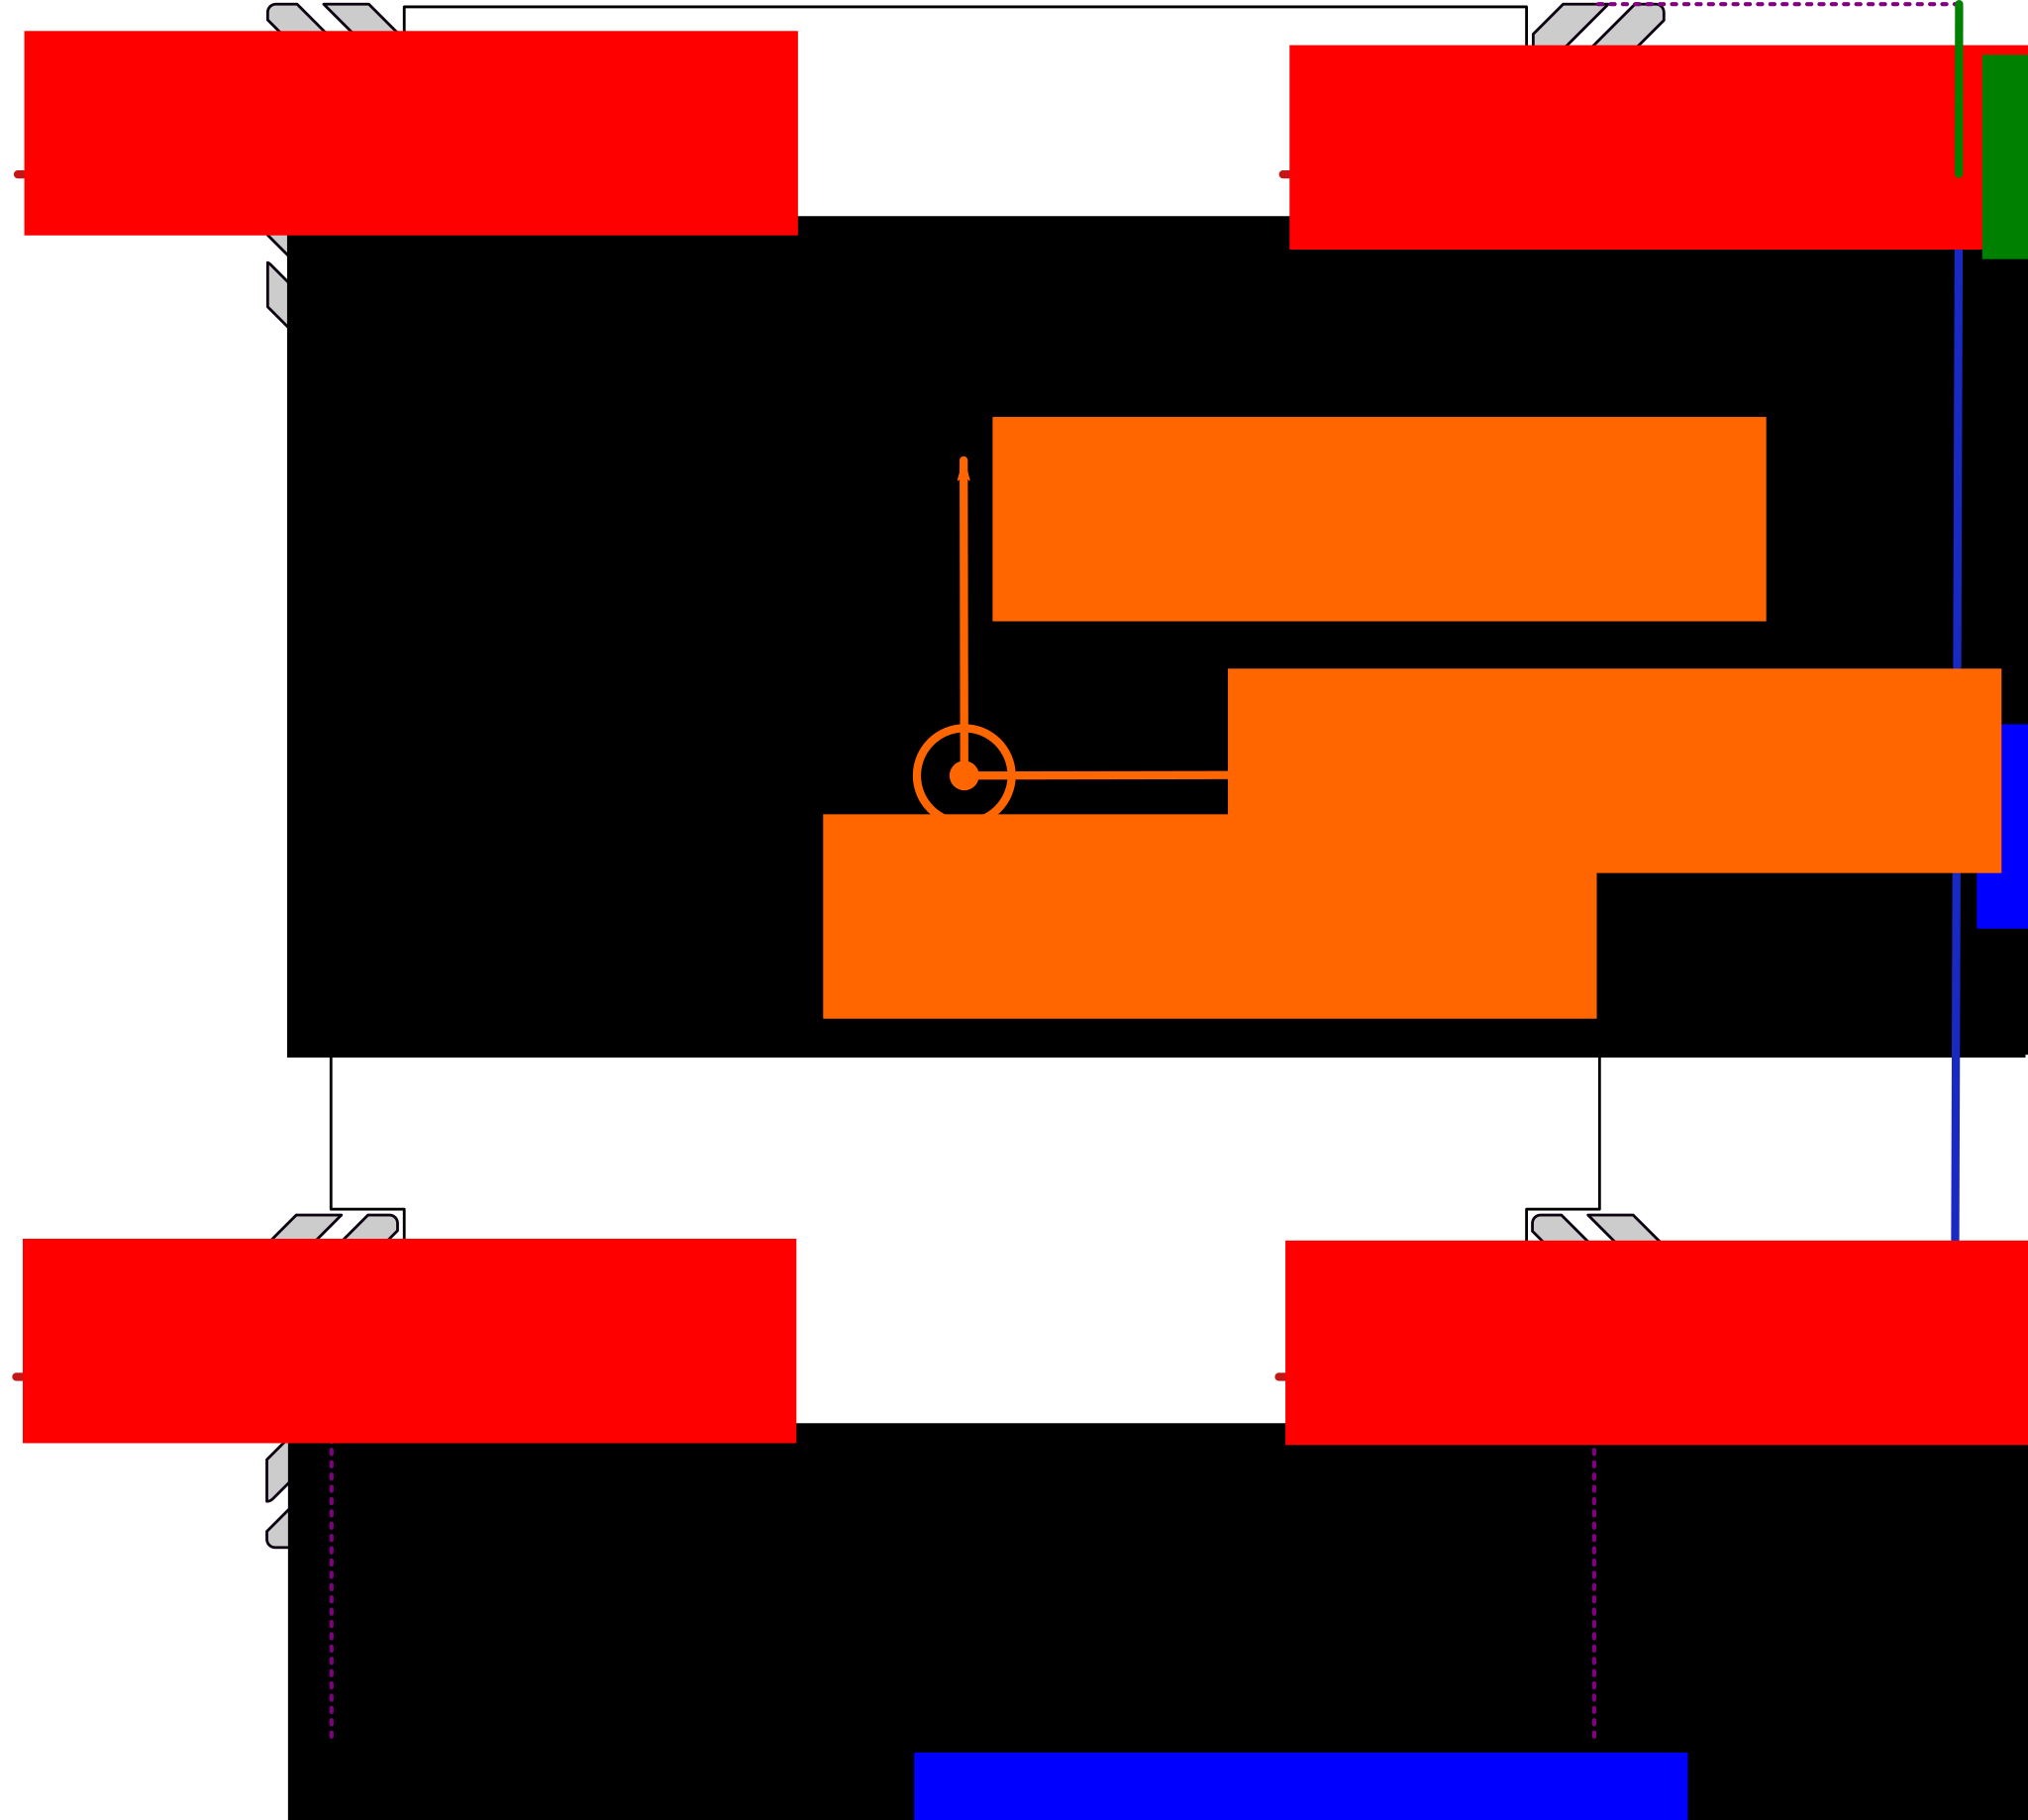
\includegraphics[width=0.5\textwidth]{graphics/base_dims.pdf} 
	\end{frame}

	\begin{frame}
		\frametitle{Czujniki}
		\begin{itemize}
			\item Enkodery generują prędkość kątową i kąt obrotu koła.
			\item Skanery laserowe zwracają przybliżony zarys obiektów wokół robota.
			\item Jednostka inercyjna mierzy przyspieszenie liniowe i prędkość kątową platformy.
		\end{itemize}
	\end{frame}
	
	
	
	\section{Model}
	\begin{frame}
		\frametitle{Składniki systemu}
		\begin{columns}[c]
			\column{0.4\textwidth}
				\centering
				\includegraphics[width=\textwidth]{graphics/model.png} \\
				Model dynamiki platformy.
			\column{0.6\textwidth}
				\begin{itemize}
					\item Uproszczony model dynamiki.
					\item Matematycznie dokładne modele kinematyki.
					\begin{itemize}
						\item Model kinematyki prostej --- koła na prędkość.
						\item Model kinematyki odwrotnej --- prędkość na koła.
					\end{itemize}
					\item Modele czujników.
					\begin{itemize}
						\item Enkodery.
						\item Skanery laserowe.
						\item Jednostki inercji.
					\end{itemize}
					\item Pakiety wspomagające testowanie.
					\begin{itemize}
						\item Generujące dane.
						\item Przyjmujące dane.
						\item Filtrujące dane.
					\end{itemize}
				\end{itemize}
		\end{columns}
	\end{frame}
	
	\begin{frame}
		\frametitle{Parametry modelu dynamiki}
		\begin{itemize}
			\item Sposób implementacji modelu.
			\item Współczynniki tarcia i poślizgu kół.
			\item Masy i momenty bezwładności ogniw.
			\item Parametry przegubów.
			\item Parametry symulatora.
		\end{itemize}
		Odpowiedni dobór parametrów pozwala na przybliżenie zachowania się modelu do platformy.

	\end{frame}

	\begin{frame}
		\frametitle{Testowanie programu sterującego}
		\centering
		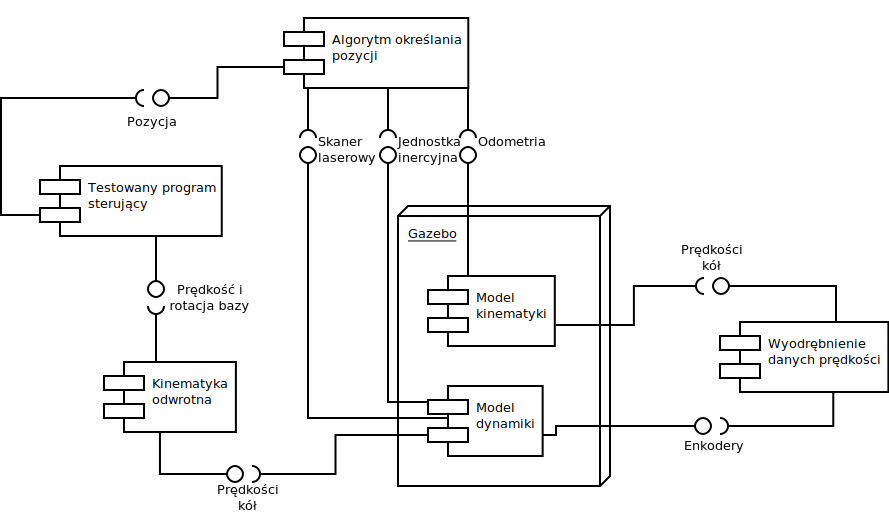
\includegraphics[width=\textwidth]{graphics/final.pdf} 
		Sposób podłączenia programu sterującego do środowiska.
	\end{frame}
	
	
	
	\section{Pomiary}
	\begin{frame}
		\frametitle{Sprzęt i wersje programów}
		Eksperymenty przeprowadzono na dobrej jakości sprzęcie i możliwie najaktualniejszych wersjach programów.
		\begin{itemize}
			\item System operacyjny Ubuntu LTS 16.04 (Xenial Xerus)
			\item ROS Kinetic Kame
		\end{itemize}
		\begin{itemize}
			\item Intel i7-4720HQ 2.60GHz
			\item 16 GiB RAM
			\item Renderowanie na wbudowanej karcie graficznej
		\end{itemize}
		W czasie testów użycie procesora nigdy nie wyniosło 100\%.
	\end{frame}
	
	\begin{frame}
		\frametitle{Porównanie modelu z platformą}
		\centering
		\includegraphics[width=\textwidth]{graphics/velmobil_xy.pdf} \\
		Prosty przebieg bez zmiany orientacji platformy.
	\end{frame}
	
	\begin{frame}
		\frametitle{Cechy modelu przy skręcie}
		\centering
		\includegraphics[width=\textwidth]{graphics/velmobil_xy_s.pdf} \\
		Przybliżenie fragmentu poprzedniego wykresu.
	\end{frame}
	
	\begin{frame}
		\frametitle{Jednostka inercyjna}
		\centering
		\includegraphics[width=\textwidth]{graphics/imu_xy.png} \\
		Porównanie rzeczywistych danych z modelem.
	\end{frame}
	
	\begin{frame}
		\frametitle{Skaner laserowy}
		\centering
		\begin{columns}[c]
			\column{0.5\textwidth}
			\centering
			\includegraphics[width=\textwidth]{graphics/screen_laser.png} \\
			Symulator
			\column{0.5\textwidth}
			\centering
			\includegraphics[width=\textwidth]{graphics/screen_rviz.png} \\
			Wizualizer danych
		\end{columns}
	\end{frame}

	
	\begin{frame}
		\frametitle{Pokaz}
		Nagrany film.
	\end{frame}
 
 
 
	\section{Podsumowanie}
	\begin{frame}
		\frametitle{Podsumowanie}
		\begin{itemize}
			\item Opracowano modele dynamiki i kinematyki.
			\item Opracowano zestaw pakietów ułatwiających przeprowadzanie testów i wizualizację.
			\item Zasymulowano czujniki modeli.
			\item Przeprowadzono testy porównujące trasy robota i modeli.
			\begin{itemize}
				\item Dobrano parametry modelu dynamiki.
				\item Dobrano parametry symulowanych czujników.
			\end{itemize}
		\end{itemize}
	\end{frame}
	\begin{frame}
		\frametitle{Perspektywy rozwoju}
		\begin{itemize}
			\item Przeprowadzenie wielokrotnych i szczegółowych testów platformy.
			\item Szczegółowa analiza modeli i symulatora oraz określenie przyczyn rozbieżności.
			\item Dobranie współczynników modeli w zautomatyzowany sposób.
			\item Badania nad zmianą implementacji modelu i symulatora.
			\item Połączenie modeli platformy i robota Velma.
		\end{itemize}
	\end{frame}
	\begin{frame}
		\frametitle{Koniec}
		\centering
		Dziękuję za uwagę.\\
		Projekt i ta prezentacja znajdują się na \url{https://github.com/Antyradek/omnivelma}.
	\end{frame}
\end{document}
